\documentclass{article}
\usepackage{graphicx} 
\usepackage{hyperref}
\usepackage{float}

\title{Advanced programming for HPC - Labwork 6}
\author{Son Dang Thai}
\date{October 2025}

\begin{document}

\maketitle

This labwork was carried out on a 512x512 image:

\begin{figure}[htbp]
    \centering
    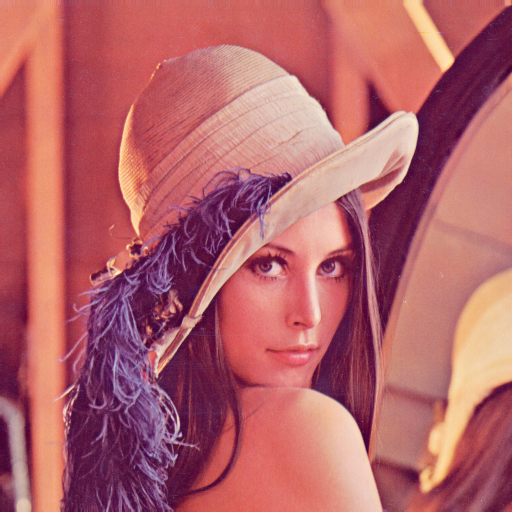
\includegraphics[width=1\linewidth]{lenna.png}
    \caption{Experiment image}
    \label{fig:Experiment image}
\end{figure}

\section{Binarization}

After loading the image to the GPU, creating a placeholder for the output image, and calculating the gray value for each pixel of the original image using the formula gray\_value = (red + green + blue) / 3, the gray value is compared with the threshold to decide which binary value it should be: 0 if it's smaller than the threshold, else 1.

In terms of the response time, with block sizes [(4, 4), (8, 8), (16, 16), (32, 32)], the response time was recorded at [0.00046515464782714844, 0.00021457672119140625, 0.00013065338134765625, 0.00012969970703125] seconds. Below is the response time graph and the result image:

\begin{figure}[H]
    \begin{minipage}{0.48\textwidth}
        \centering
        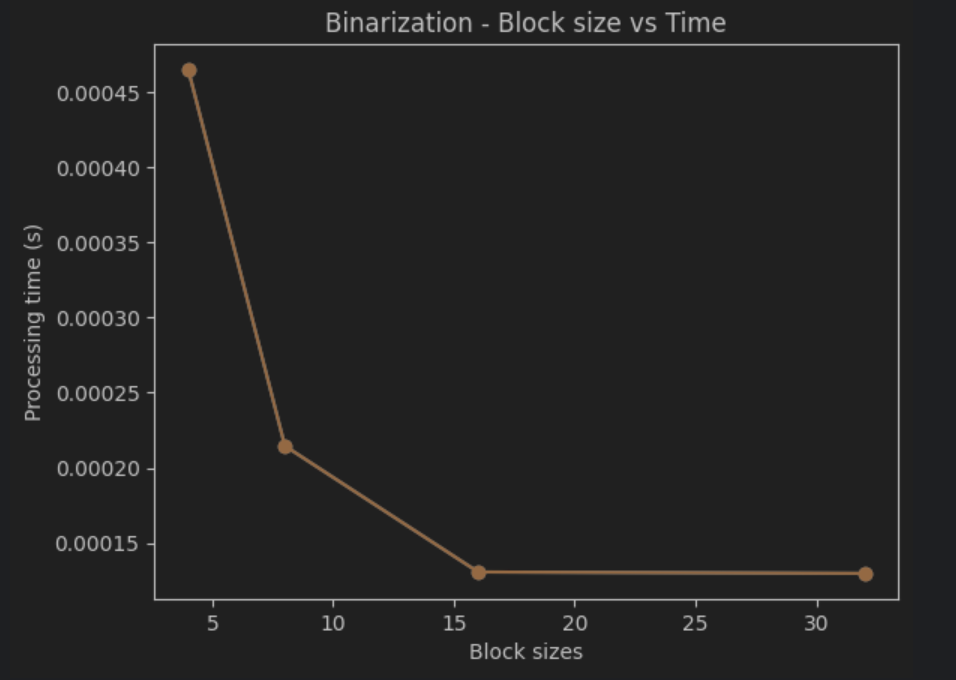
\includegraphics[width=.7\linewidth]{Binarization - Block size vs Time.png}
        \caption{Binarization graph}
        \label{fig:Binarization graph}
    \end{minipage}\hfill
    \begin{minipage}{0.48\textwidth}
        \centering
        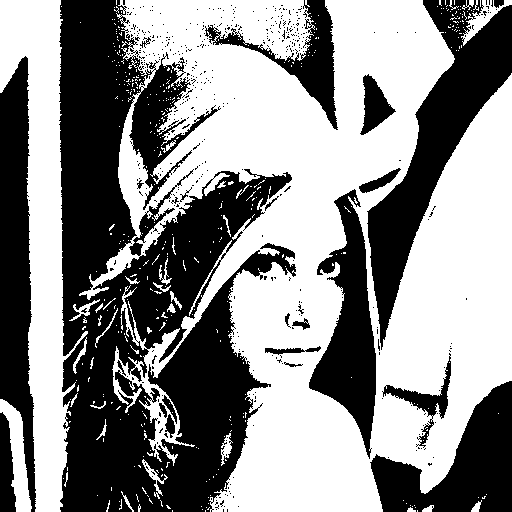
\includegraphics[width=.7\linewidth]{binarization.png}
        \caption{Binarization result}
        \label{fig:Binarization result}
    \end{minipage}\hfill
\end{figure}

This shows that the larger the block size, the shorter the response time.

\section{Brightness control}

After loading the image to the GPU and creating a placeholder for the output image, the new pixel value is calculated by the original one plus the brightness value.

In terms of the response time, with block sizes [(4, 4), (8, 8), (16, 16), (32, 32)], the response time was recorded at [0.0002455711364746094, 0.00015163421630859375, 9.441375732421875e-05, 8.606910705566406e-05] seconds. Below is the response time graph and the result image:

\begin{figure}[H]
    \begin{minipage}{0.48\textwidth}
        \centering
        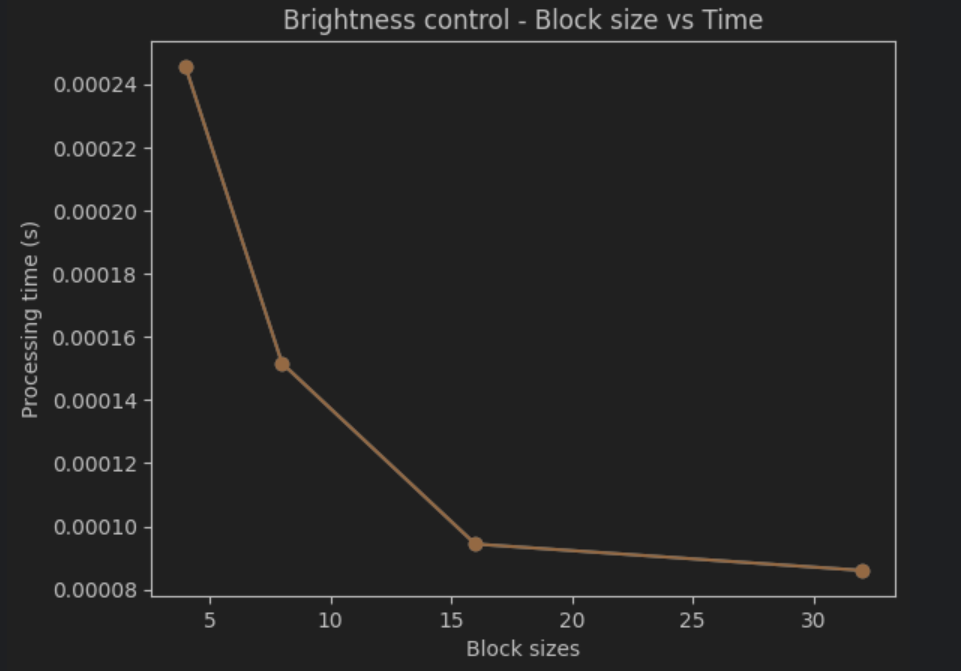
\includegraphics[width=.7\linewidth]{Brightness control - Block size vs Time.png}
        \caption{Brightness graph}
        \label{fig:Brightness graph}
    \end{minipage}\hfill
    \begin{minipage}{0.48\textwidth}
        \centering
        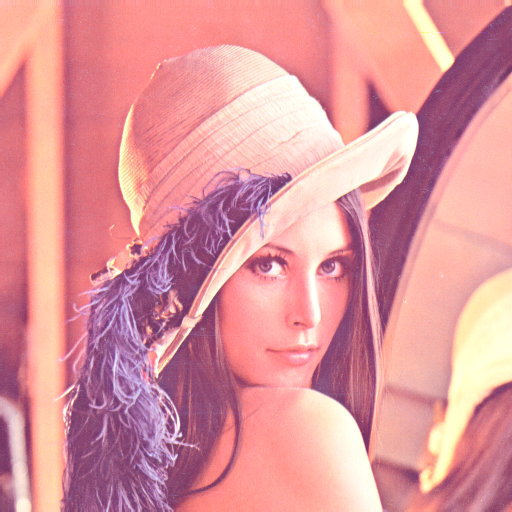
\includegraphics[width=.7\linewidth]{brightness_control.png}
        \caption{Brightness result}
        \label{fig:Brightness result}
    \end{minipage}\hfill
\end{figure}

This shows that the larger the block size, the shorter the response time.

\section{Blending images}

The second input image used here is the reversed original image. After loading the images to the GPU and creating a placeholder for the output image, the new pixel value is calculated by the formula new\_value = original\_value\_1 * weight + original\_value\_2 * (1 - weight).

In terms of the response time, with block sizes [(4, 4), (8, 8), (16, 16), (32, 32)], the response time was recorded at [0.00023794174194335938, 0.00012755393981933594, 9.179115295410156e-05, 8.082389831542969e-05] seconds. Below is the response time graph and the result image:

\begin{figure}[H]
    \begin{minipage}{0.48\textwidth}
        \centering
        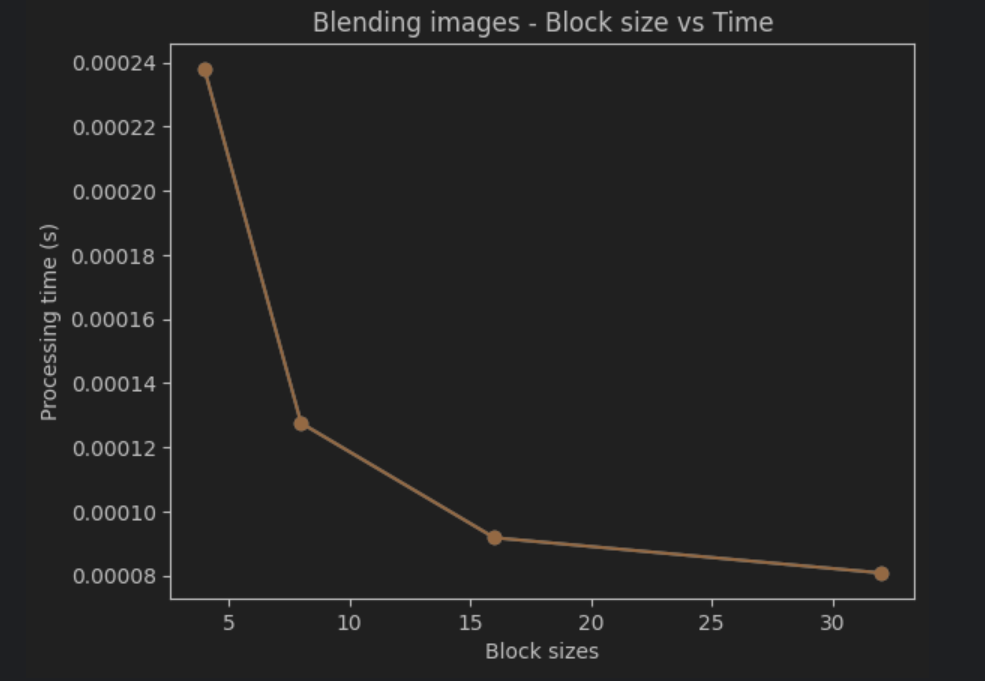
\includegraphics[width=.7\linewidth]{Blending images - Block size vs Time.png}
        \caption{Blending graph}
        \label{fig:Blending graph}
    \end{minipage}\hfill
    \begin{minipage}{0.48\textwidth}
        \centering
        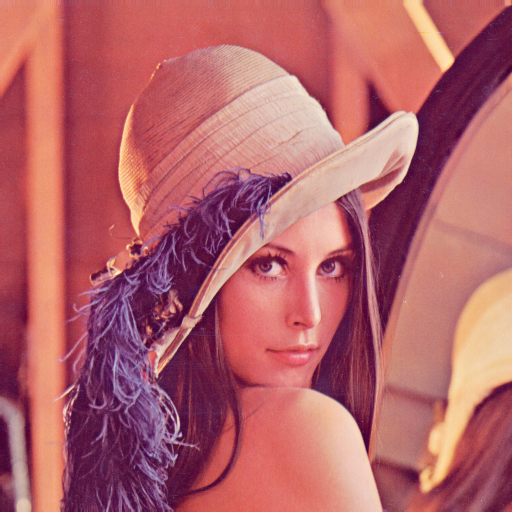
\includegraphics[width=.7\linewidth]{blending_images.png}
        \caption{Blending result}
        \label{fig:Blending result}
    \end{minipage}\hfill
\end{figure}

This shows that the larger the block size, the shorter the response time.

\end{document}
